\section{Experiments}
\label{sec:exp}

We report three outdoor comparisons on nuScenes val and one indoor comparison
on ScanNet200 val, each between the confirmation-based module and a control
granted the same output budget over shared frozen detections. Unless stated
otherwise, outdoor results use retrospective emission, whose latency cost is
$N{-}1$ observations; the corresponding frame-index delay is reported in
Sec.~\ref{sec:emissionabl}.

\subsection{Detection-budget-matched comparison}
\label{sec:detmatch}

\begin{table*}[t]
\centering\footnotesize
\setlength{\tabcolsep}{5pt}
\begin{tabular}{llrcccccccc}
\toprule
Frame & Arm & Boxes & mAP & NDS & HOTA & AssA & DetA & DetRe & IDF1 & AMOTA \\
\midrule
\multirow{4}{*}{Sensor}
 & Baseline (unfiltered)      &   718{,}786 & 0.5613 & 0.6480 & 0.1793 & 0.2007 & 0.1620 & 0.6690 & 0.1112 & 0.0858 \\
 & Control (threshold)       &   257{,}259 & \textbf{0.5504} & \textbf{0.6450} & \textbf{0.2735} & 0.2119 & \textbf{0.3570} & \textbf{0.6160} & 0.2082 & 0.0942 \\
 & Control (accumulation)     &   257{,}259 & 0.4783 & 0.6134 & 0.2604 & 0.2315 & 0.2954 & 0.5350 & 0.2146 & 0.1101 \\
 & Confirmation ($N{=}3$)     &   257{,}259 & 0.3009 & 0.5229 & 0.2462 & \textbf{0.2744} & 0.2232 & 0.4287 & 0.2054 & \textbf{0.1338} \\
\midrule
\multirow{4}{*}{World}
 & Baseline (unfiltered)      &   718{,}786 & 0.5613 & 0.6480 & 0.2837 & 0.5014 & 0.1613 & 0.6663 & 0.2715 & 0.2896 \\
 & Control (threshold)       &   517{,}566 & 0.5598 & 0.6479 & 0.3305 & 0.5146 & 0.2133 & 0.6550 & 0.3391 & 0.3137 \\
 & Control (accumulation)     &   517{,}565 & 0.5568 & 0.6467 & 0.3282 & 0.5110 & 0.2118 & 0.6511 & 0.3399 & 0.2931 \\
 & Confirmation ($N{=}3$)     &   517{,}566 & 0.4921 & 0.6200 & 0.3224 & \textbf{0.5293} & 0.1973 & 0.6141 & 0.3288 & \textbf{0.3864} \\
\bottomrule
\end{tabular}
\caption{\textbf{Detection-budget-matched comparison} on nuScenes val
($150$ scenes, frozen CenterPoint detections, retrospective emission). The
three matched arms --- a static score threshold ($0.2214$ sensor, $0.1272$
world), a confidence-accumulation control in the manner of~\cite{cbmot}, and
confirmation --- emit the same number of boxes. Bold marks the best
matched arm, omitted where the leading interval spans zero; the unfiltered
baseline is reference only and is not budget-matched.}
\label{tab:detmatch}
\end{table*}

Table~\ref{tab:detmatch} compares confirmation against controls calibrated to
the identical box count --- $257{,}259$ boxes in the sensor frame and
$517{,}566$ in the world frame, from the same frozen detector output.

\noindent\textbf{Association accuracy improves.} Against the threshold control
AssA rises from $0.2119$ to $0.2744$ in the sensor frame and from $0.5146$ to
$0.5293$ in the world frame, both intervals excluding zero
($[{+}0.0471,{+}0.0785]$ and $[{+}0.0098,{+}0.0203]$). The per-scene mean gain, a different estimator
from the difference of aggregates, is $+0.0460$; the gain holds in $113$ of
$150$ scenes
(Wilcoxon $p{=}2.6{\times}10^{-15}$, rank-biserial $0.74$).

\noindent\textbf{Class-aware tracking accuracy rises.} AMOTA goes from
$0.0942$ to $0.1338$ (sensor) and $0.3137$ to $0.3864$ (world), the largest
relative effect we measure. AMOTA admits no per-scene resampling
(Sec.~\ref{sec:stats}), so this is a point estimate that we rely on only
because it moves the same way in both frames and under the comparisons
below.

\noindent\textbf{Detection-oriented metrics fall.} At the same budget, mAP
drops $0.5504\!\to\!0.3009$ (sensor) and $0.5598\!\to\!0.4921$ (world), DetA
drops $0.3570\!\to\!0.2232$ ($[{-}0.1408,{-}0.1267]$) and
$0.2133\!\to\!0.1973$ ($[{-}0.0183,{-}0.0138]$), and detection recall drops
$0.6160\!\to\!0.4287$ ($[{-}0.2087,{-}0.1665]$) and $0.6550\!\to\!0.6141$
($[{-}0.0477,{-}0.0350]$). The DetA loss dominates the geometric mean, so
aggregate HOTA falls as well ($[{-}0.0323,{-}0.0231]$ sensor;
$[{-}0.0100,{-}0.0063]$ world).

\noindent\textbf{IDF1 shows no reliable sensor-frame difference.} The
sensor-frame interval spans zero ($[{-}0.0108,{+}0.0037]$) while the paired
per-scene test reaches significance ($p{=}7.3{\times}10^{-3}$), so the two
estimators disagree and we claim no difference; in the world frame IDF1 is
slightly \emph{lower} for the confirmation module
($[{-}0.0135,{-}0.0070]$).

\noindent\textbf{Against confidence accumulation, the two rules split the
metrics.} This control isolates \emph{which} temporal rule is used rather
than whether one is used at all. Confirmation attains higher AssA in both
frames
($0.2315\!\to\!0.2744$ sensor, $0.5110\!\to\!0.5293$ world; intervals
$[{+}0.0337,{+}0.0524]$ and $[{+}0.0146,{+}0.0225]$), and accumulation is ahead
on every other measured axis, also with intervals excluding zero: HOTA, DetA, IDF1 and DetRe
(Sec.~\ref{supp:cbmot}).
The split extends to detection quality: accumulation leads on mAP
($0.4783\!\to\!0.3009$ sensor, $0.5568\!\to\!0.4921$ world) and NDS
($0.6134\!\to\!0.5229$, $0.6467\!\to\!0.6200$).

\noindent\textbf{Scope of the accumulation control.} All statements about it
concern our reproduction under the configuration of Sec.~\ref{sec:controls},
not the original system or its published results
(Sec.~\ref{supp:cbmot}).

\subsection{Identity-budget-matched comparison}
\label{sec:idmatch}

\begin{table}[tb]
\centering\footnotesize
\setlength{\tabcolsep}{1.5pt}
\begin{tabular}{lrcccc}
\toprule
Arm & Boxes & HOTA & AssA & DetA & IDF1 \\
\midrule
\multicolumn{6}{l}{\emph{Sensor frame}} \\
Control (top-$K$)  & 190{,}708 & \textbf{0.2461} & 0.2346 & \textbf{0.2607} & \textbf{0.2081} \\
Control (rand.) & --- & --- &.2321--.2460 & --- & --- \\
Confirmation       & 360{,}309 & 0.1960 & \textbf{0.2535} & 0.1537 & 0.1531 \\
\midrule
\multicolumn{6}{l}{\emph{World frame}} \\
Control (top-$K$)  & 608{,}168 & \textbf{0.2538} & 0.4173 & \textbf{0.1553} & \textbf{0.2596} \\
Control (rand.) & --- & --- &.3878--.3934 & --- & --- \\
Confirmation       & 754{,}500 & 0.2263 & \textbf{0.4314} & 0.1196 & 0.2121 \\
\bottomrule
\end{tabular}
\caption{\textbf{Identity-budget-matched comparison.} The control keeps, per
scene, the $K$ highest-scoring tracks, $K$ being the number of identities the
confirmation module emits ($64{,}428$ sensor, $108{,}225$ world; exact in both
frames); the random-$K$ rows (``rand.'') give the range over five seeds of the
same selection made at random, scored on AssA only. The box budgets are
unequal here, in the control's disfavour on volume-sensitive metrics. AMOTA is
omitted: identity matching does not equalise class-aware evaluation volume
(Sec.~\ref{sec:stats}).}
\label{tab:idmatch}
\end{table}

Matching emitted identities rather than boxes
(Tab.~\ref{tab:idmatch}) tests whether the association gain merely reflects
having fewer identities to confuse. It does not. AssA remains higher for the
confirmation module in both frames ($0.2346\!\to\!0.2535$ sensor,
$0.4173\!\to\!0.4314$ world), with intervals excluding zero
($[{+}0.0129,{+}0.0258]$ and $[{+}0.0101,{+}0.0185]$) and per-scene wins in
$117/150$ and $111/150$ scenes ($p{=}2.2{\times}10^{-16}$ and
$4.1{\times}10^{-11}$). Selecting the same number of tracks \emph{at random}
rather than by score reproduces none of it: the seeded arms reach at most
$0.2460$ (sensor) and $0.3934$ (world), both below the confirmation module.

\noindent\textbf{The rule separation survives identity matching.} Repeating the
comparison against confidence accumulation with \emph{identities} rather than
boxes held fixed --- the accumulation control ranked by its own refined score
and cut at the confirmation module's per-scene identity count, matched exactly
--- leaves the association separation unchanged: $+0.0252$ sensor
($[{+}0.0200,{+}0.0316]$) and $+0.0172$ world ($[{+}0.0089,{+}0.0161]$),
against $+0.0253$ and $+0.0170$ at matched boxes, with the accompanying losses
on HOTA, DetA, IDF1 and DetRe keeping their sign and significance. The
separation is the same size whichever currency is held fixed, which excludes
the simplest reading of it --- that persistence gains association accuracy by
carrying fewer identities. The result is robust to the control's ranking and
matching granularity (Sec.~\ref{supp:ranking}).

\noindent\textbf{Budget asymmetry.} Identity matching necessarily leaves
unequal box counts, because score-ranked tracks are shorter than
persistence-selected ones. This biases volume-sensitive metrics against the
control --- so the AssA result here is conservative --- and we therefore read
DetA, HOTA and IDF1 from Tab.~\ref{tab:detmatch}, where boxes are matched
exactly.

\subsection{What the association gain is bought with}
\label{sec:emissionabl}

Sections~\ref{sec:detmatch} and~\ref{sec:idmatch} price confirmation in
detection retention. This section asks what \emph{else} it pays. All results so
far release a confirmed track's withheld prefix retrospectively; we first
measure the causal alternative, then a policy that avoids both costs.

\begin{table}[tb]
\centering\footnotesize
\setlength{\tabcolsep}{2.5pt}
\begin{tabular}{lrcccc}
\toprule
Arm & Boxes & mAP & HOTA & AssA & AMOTA \\
\midrule
\multicolumn{6}{l}{\emph{Sensor frame}} \\
Control (threshold)  & 221{,}297 & \textbf{0.3213} & \textbf{0.2417} & 0.2105 & 0.0574 \\
Confirmation, causal & 221{,}297 & 0.1360 & 0.2056 & \textbf{0.2861} & \textbf{0.0800} \\
\midrule
\multicolumn{6}{l}{\emph{World frame}} \\
Control (threshold)  & 503{,}619 & \textbf{0.3367} & \textbf{0.2729} & \textbf{0.4315} & 0.1825 \\
Confirmation, causal & 503{,}619 & 0.2569 & 0.2456 & 0.4199 & \textbf{0.2089} \\
\bottomrule
\end{tabular}
\caption{\textbf{Causal emission is not free either: detection-budget-matched}
($221{,}297$ boxes sensor at threshold $0.2519$, $503{,}619$ world at
$0.1539$; both arms exact). The causal arm drops the pre-confirmation prefix
instead of releasing it retrospectively. Intervals are reported for AssA only,
the metric the comparison turns on; the remaining columns are point
estimates.}
\label{tab:causal}
\end{table}

\noindent\textbf{Causal emission loses the prefix, and with it the world-frame
gain.} Table~\ref{tab:causal} repeats the detection-budget-matched comparison
with the prefix permanently dropped. The result splits by association frame.
The AMOTA gain survives in both ($0.0574\!\to\!0.0800$ sensor,
$0.1825\!\to\!0.2089$ world), and in the sensor frame the association gain is
not merely preserved but larger than under retrospective emission
($0.2105\!\to\!0.2861$; interval $[{+}0.0577,{+}0.0922]$ against
$[{+}0.0370,{+}0.0615]$ retrospectively, $110$ of $150$ scenes). In the world
frame, however, causal emission \emph{loses} association accuracy relative to
the control ($0.4315\!\to\!0.4199$), with a bootstrap interval entirely below
zero ($[{-}0.0183,{-}0.0047]$; paired $p{=}0.008$, rank-biserial $-0.25$,
confirmation ahead in only $53$ of $150$ scenes). The detection cost is larger
throughout than under retrospective emission (mAP $0.3213\!\to\!0.1360$
sensor).

Causal emission is worse where association was already easy: ego-motion
compensation leaves the world-frame control associating well on its own, and
there the discarded prefix costs more than confirmation cleans up.

\noindent\textbf{How much latency, in which unit.} The $N-1$ figure routinely
quoted for retrospective emission is correct only in observations
(Sec.~\ref{sec:latency}): over the $150$ scenes the confirmation \emph{frame}
horizon has median $3$ and $95$th percentile $7$ --- $1.5$\,s and $3.5$\,s at
the $2$\,Hz annotated-frame rate, against a constant $2$-observation horizon.
It is unbounded in principle (Sec.~\ref{supp:latency}).

\begin{table*}[t]
\centering\footnotesize
\setlength{\tabcolsep}{6pt}
\begin{tabular}{lrccccccc}
\toprule
Arm & Boxes & mAP & NDS & HOTA & AssA & DetA & IDF1 & AMOTA \\
\midrule
Baseline (ungated) & 718{,}786 & 0.5613 & 0.6480 & 0.2837 & 0.5014 & 0.1613 & 0.2715 & 0.2896 \\
Confirmation $N{=}3$ (prefix-deleting) & 368{,}724 & 0.4483 & 0.6013 & 0.3452 & 0.5265 & 0.2275 & 0.3662 & 0.4051 \\
\midrule
\multicolumn{9}{l}{\emph{Ours, provisional emission, retraction horizon $H{=}0$}} \\
\quad provisional & 295{,}403 & 0.3832 & 0.5651 & \textbf{0.3675} & \textbf{0.5619} & \textbf{0.2417} & \textbf{0.4198} & 0.3603 \\
\quad ${+}$ revision & 295{,}403 & 0.3950 & 0.5701 & --- & --- & --- & --- & 0.4200 \\
\midrule
\multicolumn{9}{l}{\emph{Ours, provisional emission, retraction horizon $H{=}4$}} \\
\quad provisional & 529{,}662 & 0.4927 & 0.6206 & 0.3219 & 0.5378 & 0.1936 & 0.3305 & 0.3823 \\
\quad ${+}$ revision & 529{,}662 & \textbf{0.5025} & \textbf{0.6247} & --- & --- & --- & --- & \textbf{0.4646} \\
\bottomrule
\end{tabular}
\caption{\textbf{Provisional emission and revision}, world frame, nuScenes val
($150$ scenes, $N{=}3$, same frozen detections and association as
Tab.~\ref{tab:detmatch}). These arms are \textbf{not budget-matched}: the box
count \emph{is} what the emission policy acts on. Revision changes no box,
score, or identity, so the class-agnostic metrics are \emph{identical} by
construction (``---''). Bold marks the best policy/confirmation value.}
\label{tab:policy}
\end{table*}

\noindent\textbf{Provisional emission retains the prefix at zero latency.}
Table~\ref{tab:policy} measures the proposed policy against the
prefix-deleting $N{=}3$ confirmation arm over the identical frozen stream. At a retraction
horizon of $H{=}4$ frames the policy emits $529{,}662$ boxes against that arm's
$368{,}724$: it retains $160{,}938$ observations ($+43.7\%$) that the arm
deletes, and it does so at an emission latency of exactly zero frames. Detection
quality on the emitted set rises accordingly (mAP $0.4483\!\to\!0.4927$, NDS
$0.6013\!\to\!0.6206$) and so does association consistency
(AssA $0.5265\!\to\!0.5378$).

\noindent\textbf{And it is not free.} Over the same comparison the policy
gives up class-agnostic detection and identity quality: DetA
$0.2275\!\to\!0.1936$, aggregate HOTA $0.3452\!\to\!0.3219$, IDF1
$0.3662\!\to\!0.3305$, and AMOTA before revision falls
$0.4051\!\to\!0.3823$. Emitting a provisional record means emitting records
that causal confirmation would have suppressed and that ground truth does not support, and
the class-agnostic metrics price exactly that.

\noindent\textbf{Revision recovers the class-aware endpoint.} Applying the
completed-evidence label to the already-emitted stream takes AMOTA
$0.3823\!\to\!0.4646$ at $H{=}4$ ($+0.0823$), leaving the net effect against
the prefix-deleting confirmation arm at $+0.0594$: revision restores, and then
exceeds, an AMOTA the emission step had lost rather than adding one on top of
it. It says nothing about association --- the class-agnostic matcher does not
read the class label, so those columns are a mechanical identity, not a null
result.

\noindent\textbf{The retraction horizon saturates.} $H$ prices how long a
provisional record may still be withdrawn. At $H{=}4$ the emitted output
becomes identical --- byte-identical, verified by checksum --- to the
unbounded $H{=}\infty$ policy that defers the decision to scene end, because no
track that ever confirms has a pre-confirmation gap wider than four frames.
Every endpoint at $H\!\ge\!4$ therefore coincides by output equality rather
than by a tuned metric match. The bound replaces the scene-end decision at no cost
in output (Sec.~\ref{supp:horizon}).

\noindent\textbf{The horizon is itself a trade-off.} Tightening it to $H{=}0$
--- retract at the first missed frame --- reverses the picture: the policy then
emits fewer boxes than the confirmation arm ($295{,}403$) and is the \emph{best} arm in the
table on every class-agnostic metric (AssA $0.5619$, HOTA $0.3675$, DetA
$0.2417$, IDF1 $0.4198$), while giving up mAP and AMOTA. We report both
endpoints rather than selecting the one that flatters a chosen column: $H$
buys retention and detection quality with class-agnostic identity quality,
and $H{=}4$ is the setting at which the unbounded-horizon result is recovered
in full at bounded latency.



\subsection{Confirmation-window sensitivity}
\label{sec:nsweep}

% Confirmation-window trade-off curve. Numbers are Tab. tab:nsweep (supplementary).
% Requires pgfplots (loaded in main.tex).
\begin{figure}[t]
\centering
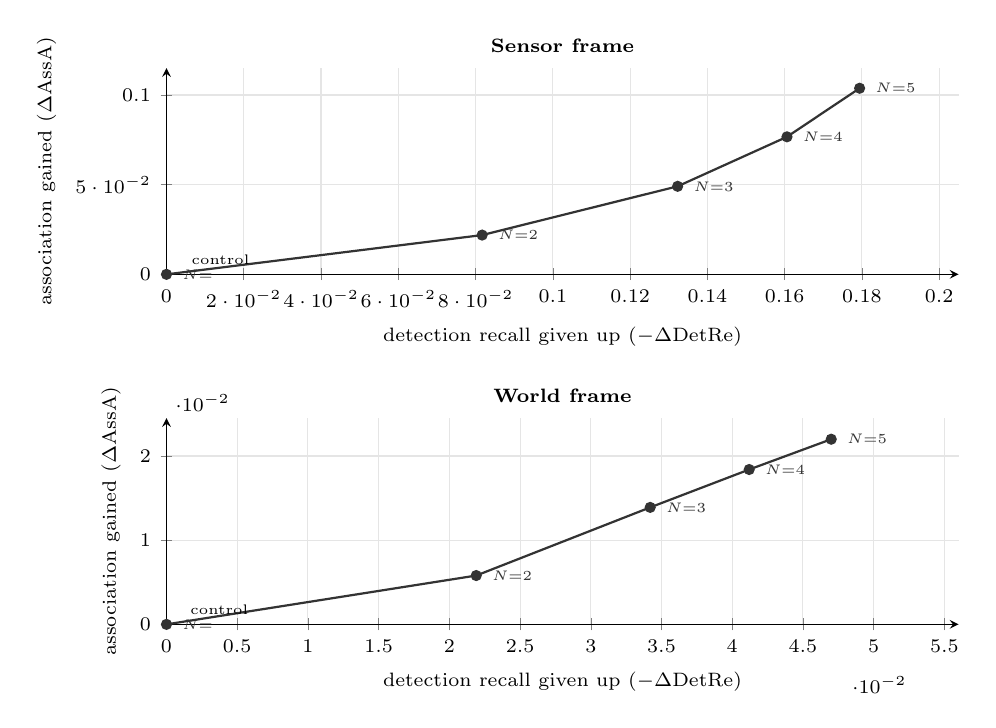
\begin{tikzpicture}
\pgfplotsset{
  every axis/.append style={
    width=0.96\linewidth, height=4.2cm,
    tick label style={font=\scriptsize}, label style={font=\scriptsize},
    title style={font=\scriptsize\bfseries, yshift=-2pt},
    axis lines=left, xmin=0, ymin=0,
    grid=major, grid style={gray!20},
  },
  every node near coord/.append style={font=\tiny, anchor=west, xshift=1pt},
}
\begin{axis}[
  name=sensor, title={Sensor frame},
  xmax=0.205, ymax=0.115,
  xlabel={detection recall given up ($-\Delta$DetRe)},
  ylabel={association gained ($\Delta$AssA)},
]
\addplot[thick, mark=*, mark size=1.6pt, color=black!80,
         nodes near coords={$N{=}\pgfplotspointmeta$}, point meta=explicit symbolic]
  coordinates {(0,0)[\!\!] (0.0817,0.0219)[2] (0.1323,0.0491)[3]
               (0.1606,0.0767)[4] (0.1794,0.1038)[5]};
\node[font=\tiny, anchor=south west] at (axis cs:0.004,0.0) {control};
\end{axis}
\begin{axis}[
  at={(sensor.below south west)}, anchor=north west, yshift=-8mm,
  title={World frame},
  xmax=0.056, ymax=0.0245,
  xlabel={detection recall given up ($-\Delta$DetRe)},
  ylabel={association gained ($\Delta$AssA)},
]
\addplot[thick, mark=*, mark size=1.6pt, color=black!80,
         nodes near coords={$N{=}\pgfplotspointmeta$}, point meta=explicit symbolic]
  coordinates {(0,0)[\!\!] (0.0219,0.0058)[2] (0.0342,0.0139)[3]
               (0.0412,0.0184)[4] (0.0470,0.0220)[5]};
\node[font=\tiny, anchor=south west] at (axis cs:0.001,0.0) {control};
\end{axis}
\end{tikzpicture}
\caption{\textbf{Confirmation is a trade-off curve, not a tuned setting.} Each
point is confirmation at that $N$ minus \emph{its own} detection-budget-matched
threshold control, so the control sits at the origin. Moving right along the
curve spends detection recall and $N{-}1$ frames of latency ($0.5$\,s each at
$2$\,Hz) and buys association accuracy; $N$ is chosen by the latency a
deployment can absorb rather than by a metric. The association gain is
positive at every $N$ in both frames and all eight bootstrap intervals exclude
zero. Full numbers, including intervals and $\Delta$AMOTA --- which, unlike
$\Delta$AssA, turns over inside the range --- are in the supplementary.}
\label{fig:nsweep}
\end{figure}


All results so far fix $N{=}3$. Figure~\ref{fig:nsweep} varies it over
$\{2,3,4,5\}$, giving each $N$ its own exactly matched control, and asks what
the choice is worth. $N{=}1$ is excluded: it reproduces the unfiltered baseline
detection-for-detection, so its matched control is the same box set and every
difference is zero by construction.

The association gain does not depend on the operating point. It is positive at
every $N$ in both association frames, and all eight intervals exclude zero. It
also grows monotonically with $N$, close to linearly in the sensor frame and
with visible deceleration in the world frame, while AMOTA flattens in the
sensor frame and turns over in the world frame, peaking at $N{=}4$
(Tab.~\ref{tab:nsweep}). The
detection cost, meanwhile, rises without turning over at any $N$ we measured,
and the latency rises linearly by construction.

No single $N$ in this range is best on every metric, and $N{=}3$ is not the
best on any of them. We report this rather than adjust the operating point:
re-selecting $N$ from the sweep would convert an inherited constant into a
value tuned on the test metrics, the practice the matched controls exist to
guard against. We keep $N{=}3$ because $N$ is a latency budget, not a tuned
hyperparameter: it is fixed by the $N{-}1$ observations of delay a deployment
can absorb. What the sweep establishes is that the consistency gain is a
property of confirmation over the whole range tested, not an artifact of one
setting, and that larger windows buy more of it at proportionally more
detection cost and latency. The widening gap is driven by the confirmed arm
rather than by a failing control, whose own AssA also rises as the matched
budget tightens (Tab.~\ref{tab:nsweep}).

\subsection{Indoor: semantic stability}
\label{sec:indoor}

\begin{table}[tb]
\centering\footnotesize
\setlength{\tabcolsep}{2pt}
\begin{tabular}{lrrcc}
\toprule
Arm & Inst. & Switches & AP & AP$_{50}$ \\
\midrule
Baseline (unfiltered)  & --- & --- & 0.1956 & --- \\
Control (top-$K$)      & 10{,}410 & 23{,}303 & 0.1926 & 0.2504 \\
Control (random $K$)   & --- & 23{,}275--23{,}288 & --- & --- \\
Confirmation ($N{=}3$) & 10{,}413 & \textbf{17{,}045} & 0.1954 & 0.2532 \\
\bottomrule
\end{tabular}
% TODO(pending indoor re-run): add a "Switches / opportunity" rate column.
% Denominator now logged by scripts/indoor_matched_control.py (n_obs_total -
% n_unique_total); it falls out of the indoor N-sweep run at no extra cost.
\caption{\textbf{Indoor comparison} on ScanNet200 val ($312$ scenes, frozen
Mask3D proposals with per-frame open-vocabulary labels). The primary endpoint
is the per-scene label-switch count (lower is better, bold); the control keeps
the $K$ highest-scoring instances per scene, $K$ matched to the confirmation
module's emitted-instance count, and the random-$K$ row spans three seeds
($23{,}275$, $23{,}277$, $23{,}288$). The AP columns are secondary and untested.
The unfiltered baseline is a validity anchor rather than an arm, and only its
AP was recorded, hence its empty cells.}
\label{tab:indoor}
\end{table}

The indoor experiment asks whether the same rule improves \emph{semantic}
stability in the pipeline of Sec.~\ref{sec:datasets}, which shares nothing with
the outdoor one. Against the identity-matched control, confirmation reduces label
switches from $23{,}303$ to $17{,}045$, a $26.9\%$ reduction at an essentially
equal instance budget ($10{,}413$ vs.\ $10{,}410$). The reduction is $18.0$ switches at the median
(Sec.~\ref{supp:indoor}) and holds in $309$ of $312$ scenes (Wilcoxon
$p{=}1.5{\times}10^{-52}$, rank-biserial $0.99$). The three random-$K$ arms are
indistinguishable from the score-ranked control and far from the confirmation
module, so the reduction is specific to temporal selection rather than to
emitting fewer instances by any rule.

The secondary endpoint shows no material change: AP $0.1954$ against $0.1956$
unfiltered and $0.1926$ for the control. Unlike outdoors, the indoor gain
therefore does not come at a measurable detection-quality cost --- the two
pipelines differ in whether the withheld detections carry segmentation mass,
and we report the difference in effect without claiming the outdoor trade-off
is avoidable in general.


\section{Discussion}
\label{sec:discussion}

\subsection{Confirmation is a trade-off, not a free gain}

Against an unfiltered baseline, temporal confirmation appears to improve
nearly every tracking metric. Against a non-temporal rule granted the same
output budget, most of that apparent improvement is the effect of emitting
less, and what survives is both sharper and smaller: association consistency
improves, and detection-oriented accuracy degrades over an \emph{identical}
box set. The gain is bought rather than added, and each additional observation
of delay buys more of it at proportionally more detection cost. Against
confidence accumulation the picture is a split rather than an ordering ---
persistence takes association consistency, accumulation keeps the detection-
and identity-oriented measures --- so the choice between them is a choice of
which axis a system is consumed along, not a ranking.

\subsection{Provisional emission changes the currency of the cost}

Confirmation must decide what to do with the observations that precede it, and
the classical rule offers only two answers: release them late, or drop them
and lose the world-frame association gain with them. Neither is compatible
with a consumer that must act immediately on output whose reliability improves
later. The policy's content is a separation --- \emph{when output becomes
available} is decoupled from \emph{when evidence becomes reliable} --- which
converts the currency of the cost from latency or retention into
revisability: the consumer must accept that a record it holds may be updated
or withdrawn, and the retraction horizon bounds how long that obligation
lasts. It is an operating-point change, not a new confirmation mechanism.

\subsection{Limitations}

\noindent\textbf{The revision endpoint is single.} AMOTA is the only
class-aware metric available to us; the class-agnostic family cannot respond
to a semantic-only change, and its invariance in Tab.~\ref{tab:policy} is
mechanical rather than a null result. Whether revision affects identity
consistency would need a class-aware association metric, which we do not have
and do not claim. Nor do we separate the label change from the nuScenes
attribute recomputation it entails, so the AMOTA gain is attributed to the
pair.

\noindent\textbf{Scope.} We do not measure what a downstream planner or mapper
pays to apply a revision or a retraction. The full tracking evaluation is
nuScenes only, over a single frozen CenterPoint detection set, so we make no
cross-detector claim; ScanNet200 has no instance-tracking ground truth, so the
indoor endpoint is label switching rather than an identity metric and tests
whether the confirmation rule transfers, not whether the streaming claim holds
there.

\section{Conclusion}
\label{sec:conclusion}

Temporal confirmation provides a genuine association-consistency gain under
matched detection and identity budgets, but the gain is coupled to detection
retention and to latency. Provisional emission separates immediate output from
evidence maturity: observations are emitted causally, then revised or retracted
as evidence accumulates. On nuScenes, $H{=}4$ retains $43.7\%$ more
observations than the prefix-deleting confirmation arm and revision raises
AMOTA by $0.0823$ over the provisional output. Against the prefix-deleting arm
the policy gives up class-agnostic detection and identity quality. On
ScanNet200 the same rule reduces class-label switching by $26.9\%$ at a matched
identity count.
Confirmation is therefore best understood as an operating point in a
detection--association--latency--revisability trade-off rather than a
uniformly better tracker.
